\chapter{Исследовательская часть}

В данном разделе будут приведены примеры работы программы, проведен сравнительный анализ алгоритмов при различных ситуациях на основе полученных данных и проведена параметризация реализации муравьиного алгоритма.

\section{Технические характеристики}

Технические характеристики устройства, на котором выполнялся эксперимент представлены далее:

\begin{enumerate}[label=\arabic*)]
	\item операционная система --- Ubuntu 22.04.3~\cite{ubuntu} Linux x86\_64;
	\item память --- 16 Гб;
	\item процессор --- Intel® Core™ i5-1135G7 @ 2.40 ГГц.
\end{enumerate}

При эксперименте ноутбук не был включен в сеть электропитания.

\section{Демонстрация работы программы}

На рисунке~\ref{fig:example} представлен пример работы программы для обоих алгоритмов --- полного перебора и муравьиного.

\begin{figure}[h!]
	\centering
	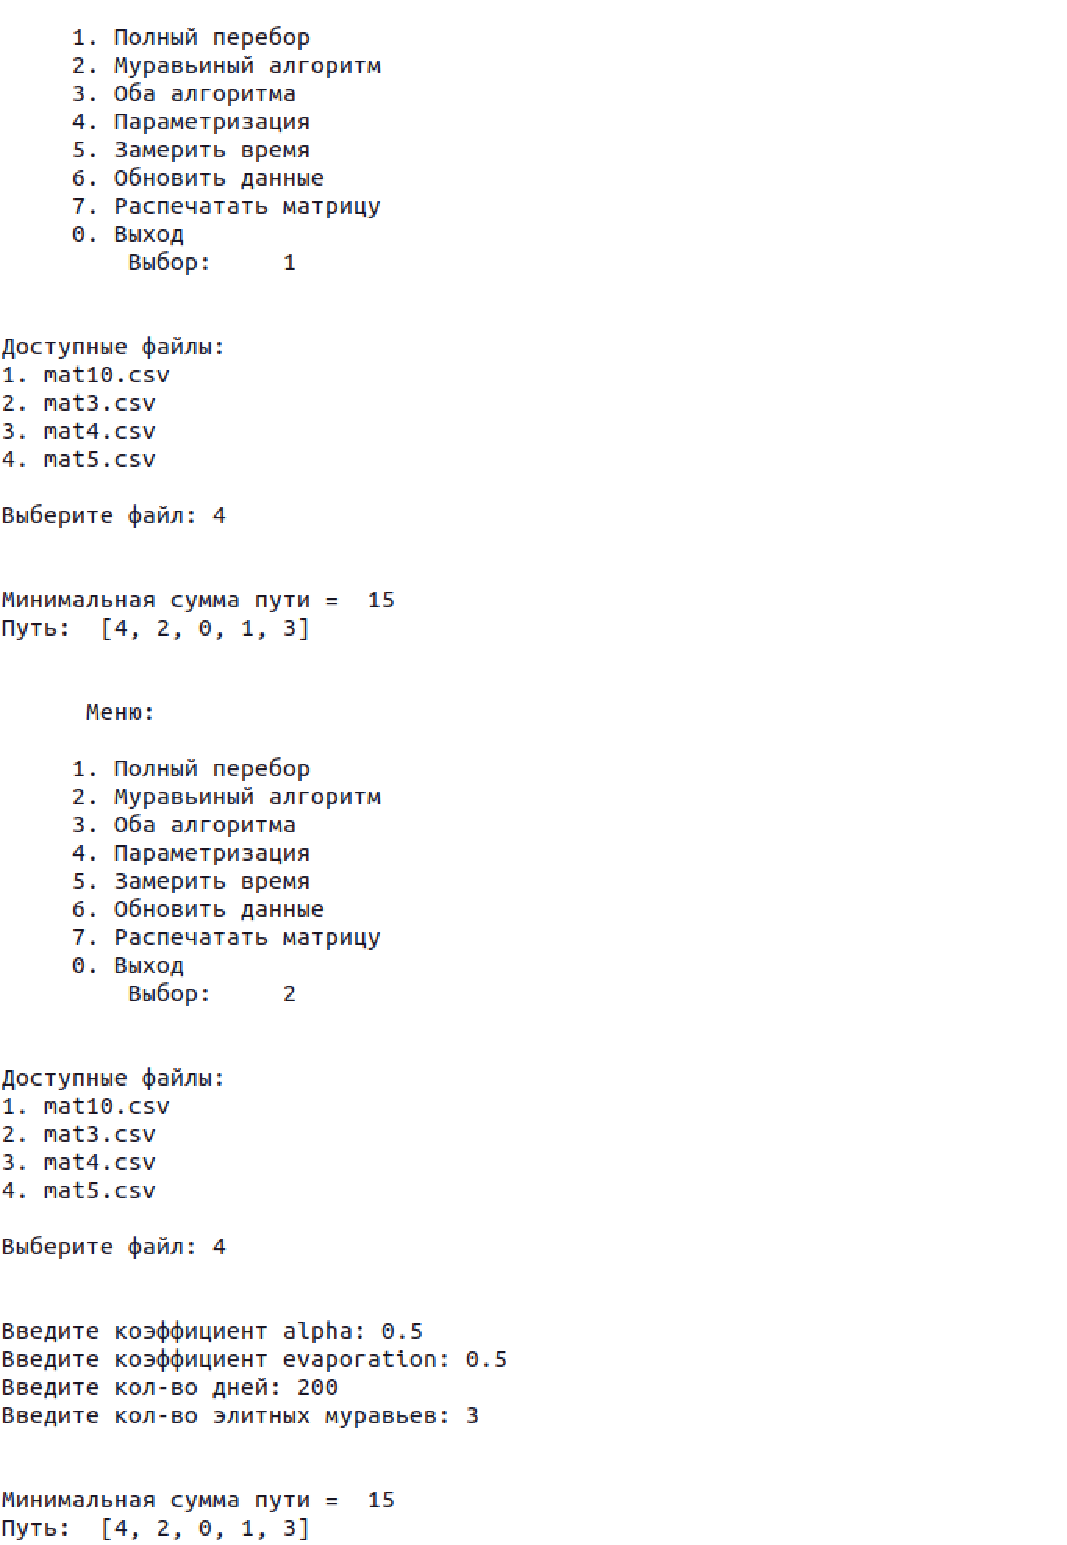
\includegraphics[width=0.95\linewidth]{img/example}
	\caption{Пример работы программы}
	\label{fig:example}
\end{figure}
\clearpage

\section{Время выполнения реализаций алгоритмов}

Как было сказано выше, используется функция замера процессорного времени  \textit{process\_time(...)} из библиотеки \textit{time} на \textit{Python}. Функция возвращает процессорное время типа float в секундах.

Функция используется дважды: перед началом выполнения алгоритма и после завершения, затем из конечного времени вычитается начальное, чтобы получить результат.

Замеры проводились для разного размера матриц, чтобы определить, когда наиболее эффективно использовать муравьиный алгоритм.

Результаты замеров приведены в таблице \ref{tbl:time_mes} (время в с).


\begin{center}
\captionsetup{justification=raggedright,singlelinecheck=off}
\begin{longtable}[c]{|r|r|r|}
\caption{Результаты замеров времени\label{tbl:time_mes}}\\ \hline
    Размер & Полный перебор & Муравьиный алгоритм \\ \hline
        2 &     0.0000 &     0.0023 \\ \hline
        3 &     0.0000 &     0.0072 \\ \hline
        4 &     0.0001 &     0.0184 \\ \hline
        5 &     0.0002 &     0.0385 \\ \hline
        6 &     0.0014 &     0.0718 \\ \hline
        7 &     0.0113 &     0.1202 \\ \hline
        8 &     0.1090 &     0.1873 \\ \hline
        9 &     1.1419 &     0.2825 \\ \hline
        10 &    12.7923 &     0.4079 \\ \hline
        
\end{longtable}
\end{center}
\clearpage


Также на рисунке \ref{fig:graph} приведены графические результаты замеров.

\begin{figure}[h!]
	\centering
	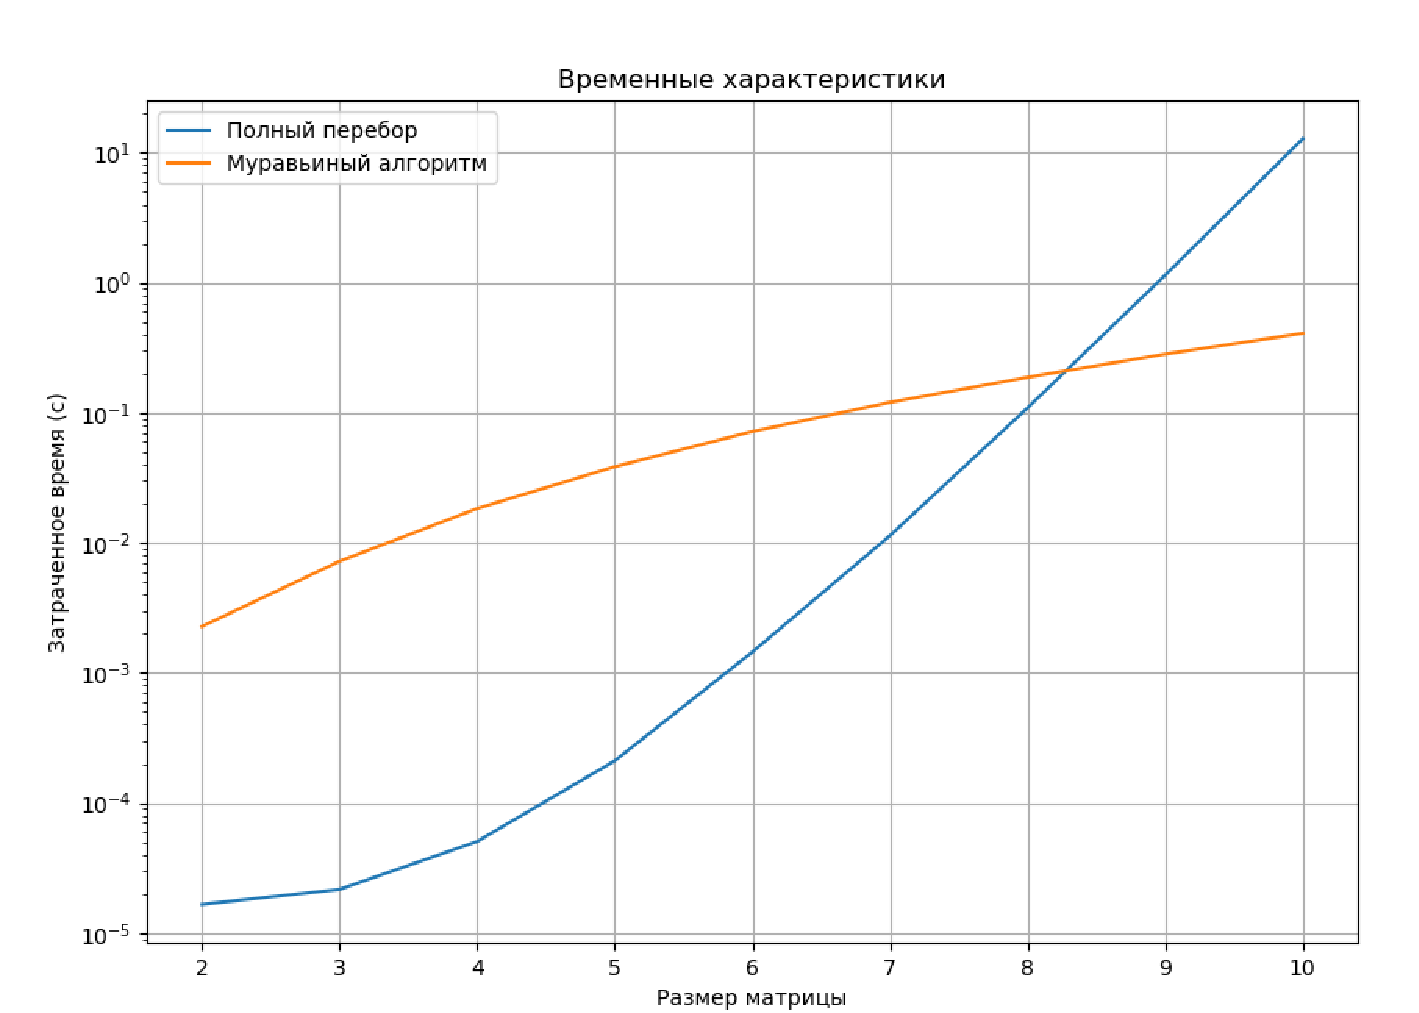
\includegraphics[width=0.95\linewidth]{img/graph}
	\caption{Сравнение по времени алгоритмов полного перебора путей и муравьиного на разных размерах матрицы}
	\label{fig:graph}
\end{figure}


\section{Постановка эксперимента}

Автоматическая параметризация была проведена на трех классах данных --- \ref{eq:kd1} -- \ref{eq:kd3}. Алгоритм будет запущен для всех значений $\alpha, \rho \in (0, 1), days = \{1, 3, 5, 10, 50, 100, 300, 500\}, e = \{3, 10, 20\}$.

Итоговая таблица значений параметризации будет состоять из следующих колонок:
\begin{itemize}
    \item $\alpha$ --- изменяющийся параметр;
    \item $\rho$ --- изменяющийся параметр;
    \item \textit{days} --- кол-во дней, изменяющийся параметр;
    \item \textit{e} --- кол-во элитных муравьев;
    \item \textit{Result} --- эталонный результат;
    \item \textit{Mistake} --- разность получившегося значения и эталонного значения на данных значениях параметров.
\end{itemize}

\textit{Цель эксперимента} --- определить комбинацию параметров, которые решают задачу наилучшим образом. Качество зависит от двух факторов:
\begin{itemize}
    \item количества дней;
    \item погрешности измерений.
\end{itemize}

\subsection{Класс данных}

Класс данных состоит из 3 матриц смежности размером 10 элементов (\ref{eq:kd1}--\ref{eq:kd3}).

\begin{equation}
    \label{eq:kd1}
	K_{1} = \begin{pmatrix}
		0 & 14 & 1 & 3 & 4 & 26 & 23 & 20 & 21 & 15 \\
		21 & 0 & 25 & 19 & 19 & 16 & 7 & 15 & 8 & 7 \\
		24 & 30 & 0 & 24 & 28 & 5 & 10 & 20 & 25 & 15 \\
		20 & 2 & 23 & 0 & 26 & 20 & 21 & 2 & 17 & 23 \\
		27 & 24 & 17 & 18 & 0 & 17 & 27 & 15 & 23 & 6 \\
		13 & 19 & 1 & 20 & 22 & 0 & 20 & 14 & 21 & 6 \\
		12 & 10 & 10 & 19 & 19 & 26 & 0 & 12 & 24 & 16 \\
		4 & 8 & 17 & 10 & 19 & 5 & 3 & 0 & 22 & 29 \\
		10 & 9 & 20 & 21 & 21 & 28 & 7 & 19 & 0 & 19 \\
		23 & 13 & 29 & 9 & 15 & 1 & 2 & 22 & 5 & 0 \\
	\end{pmatrix}
\end{equation}


\begin{equation}
	\label{eq:kd2}
	K_{2} = \begin{pmatrix}
		0 & 15 & 8 & 24 & 18 & 5 & 28 & 18 & 27 & 25 \\
		17 & 0 & 6 & 13 & 13 & 16 & 27 & 17 & 1 & 2 \\
		2 & 24 & 0 & 19 & 9 & 3 & 25 & 2 & 13 & 26 \\
		20 & 21 & 29 & 0 & 14 & 13 & 22 & 7 & 18 & 28 \\
		21 & 18 & 26 & 18 & 0 & 15 & 30 & 8 & 21 & 5 \\
		9 & 3 & 6 & 30 & 23 & 0 & 2 & 22 & 24 & 23 \\
		26 & 7 & 26 & 27 & 11 & 12 & 0 & 5 & 25 & 2 \\
		4 & 16 & 15 & 28 & 28 & 19 & 4 & 0 & 20 & 28 \\
		22 & 22 & 11 & 23 & 12 & 30 & 16 & 30 & 0 & 16 \\
		20 & 16 & 10 & 16 & 20 & 13 & 3 & 30 & 20 & 0 \\
	\end{pmatrix}
\end{equation}

\begin{equation}
	\label{eq:kd3}
	K_{3} = \begin{pmatrix}
		0 & 20 & 2 & 24 & 18 & 23 & 27 & 24 & 17 & 28 \\
		25 & 0 & 10 & 1 & 29 & 18 & 3 & 26 & 6 & 20 \\
		1 & 12 & 0 & 14 & 16 & 28 & 9 & 15 & 24 & 30 \\
		15 & 12 & 27 & 0 & 20 & 9 & 25 & 24 & 26 & 30 \\
		1 & 6 & 11 & 2 & 0 & 8 & 12 & 21 & 12 & 5 \\
		7 & 10 & 14 & 5 & 9 & 0 & 5 & 15 & 5 & 17 \\
		15 & 29 & 11 & 18 & 20 & 3 & 0 & 17 & 23 & 28 \\
		2 & 16 & 22 & 8 & 26 & 11 & 8 & 0 & 29 & 25 \\
		15 & 6 & 5 & 14 & 20 & 9 & 25 & 8 & 0 & 11 \\
		8 & 17 & 4 & 2 & 24 & 11 & 7 & 2 & 14 & 0 \\
	\end{pmatrix}
\end{equation}

Для каждой таблицы смежности из класса данных приведена таблица с выборкой параметров, которые наилучшим образом решают поставленную задачу --- (\ref{tbl:table_kd1}--\ref{tbl:table_kd3}).

\begin{center}
    \captionsetup{justification=raggedright,singlelinecheck=off}
    \begin{longtable}[c]{|c|c|c|c|c|c|}
    \caption{Параметризация для класса данных 1\label{tbl:table_kd1}} 
    	\\ \hline
        $\alpha$ & $\rho$ & Days & e & Result & Mistake \\ \hline
        0.1 &  0.1 &  500 &    3 &    45 & 0 \\ \hline
        0.1 &  0.2 &  500 &   20 &    45 &     0 \\ \hline
        0.1 &  0.3 &  500 &    3 &    45 &     0 \\ \hline
        0.1 &  0.3 &  500 &   10 &    45 &     0 \\ \hline
        0.1 &  0.5 &  100 &   20 &    45 &     0 \\ \hline
        0.1 &  0.5 &  500 &   20 &    45 &     0 \\ \hline
        0.1 &  0.8 &  500 &   10 &    45 &     0 \\ \hline
        0.2 &  0.1 &  500 &   20 &    45 &     0 \\ \hline
        0.2 &  0.2 &  500 &   10 &    45 &     0 \\ \hline
        0.2 &  0.3 &  300 &   20 &    45 &     0 \\ \hline
        0.2 &  0.4 &  500 &    3 &    45 &     0 \\ \hline
        0.2 &  0.5 &  300 &   10 &    45 &     0 \\ \hline
        0.2 &  0.7 &  100 &   10 &    45 &     0 \\ \hline
        0.2 &  0.8 &  300 &    3 &    45 &     0 \\ \hline
        0.2 &  0.8 &  300 &   10 &    45 &     0 \\ \hline
        0.3 &  0.3 &  300 &   10 &    45 &     0 \\ \hline
        0.3 &  0.3 &  300 &   20 &    45 &     0 \\ \hline
        0.3 &  0.5 &  500 &   20 &    45 &     0 \\ \hline
        0.4 &  0.2 &  300 &   20 &    45 &     0 \\ \hline
        0.4 &  0.8 &  500 &    3 &    45 &     0 \\ \hline
        0.5 &  0.4 &  300 &   10 &    45 &     0 \\ \hline
        0.5 &  0.5 &  500 &   10 &    45 &     0 \\ \hline
        0.5 &  0.6 &   50 &    3 &    45 &     0 \\ \hline
        0.6 &  0.2 &  500 &   20 &    45 &     0 \\ \hline
        0.6 &  0.4 &  500 &    3 &    45 &     0 \\ \hline
        0.6 &  0.7 &   50 &   10 &    45 &     0 \\ \hline
        0.7 &  0.5 &  300 &    3 &    45 &     0 \\ \hline 
        0.8 &  0.2 &  300 &   10 &    45 &     0 \\ \hline
        0.8 &  0.4 &  100 &   20 &    45 &     0 \\ \hline
        0.8 &  0.5 &  300 &   20 &    45 &     0 \\ \hline
\end{longtable}
\end{center}


\begin{center}
    \captionsetup{justification=raggedright,singlelinecheck=off}
    \begin{longtable}[c]{|c|c|c|c|c|c|}
    \caption{Параметризация для класса данных 2\label{tbl:table_kd2}}\\ \hline
        $\alpha$ & $\rho$ & Days & e & Result & Mistake \\ \hline
        0.1 &  0.1 &  500 &   10 &    46 &     0 \\ \hline
        0.1 &  0.2 &  100 &   20 &    46 &     0 \\ \hline
        0.1 &  0.2 &  500 &    3 &    46 &     0 \\ \hline
        0.1 &  0.3 &  100 &    3 &    46 &     0 \\ \hline
        0.1 &  0.4 &  500 &   20 &    46 &     0 \\ \hline
        0.1 &  0.5 &  100 &   10 &    46 &     0 \\ \hline
        0.1 &  0.5 &  500 &    3 &    46 &     0 \\ \hline
        0.1 &  0.6 &  500 &   20 &    46 &     0 \\ \hline
        0.1 &  0.7 &  300 &    3 &    46 &     0 \\ \hline
        0.1 & 0.7 & 500 & 10 & 46 & 0 \\ \hline
        0.1 & 0.8 & 500 & 10 & 46 & 0 \\ \hline
        0.2 & 0.1 & 500 & 10 & 46 & 0 \\ \hline
        0.2 & 0.2 & 100 & 10 & 46 & 0 \\ \hline
        0.2 & 0.2 & 500 & 3 & 46 & 0 \\ \hline
        0.2 & 0.4 & 300 & 3 & 46 & 0 \\ \hline
        0.2 & 0.6 & 500 & 10 & 46 & 0 \\ \hline
        0.2 & 0.7 & 50 & 3 & 46 & 0 \\ \hline
        0.2 & 0.8 & 50 & 3 & 46 & 0 \\ \hline
        0.2 & 0.8 & 50 & 20 & 46 & 0 \\ \hline
        0.3 & 0.1 & 300 & 20 & 46 & 0 \\ \hline
        0.3 & 0.1 & 500 & 3 & 46 & 0 \\ \hline
        0.3 & 0.2 & 500 & 10 & 46 & 0 \\ \hline
        0.3 & 0.2 & 500 & 20 & 46 & 0 \\ \hline
        0.3 & 0.3 & 50 & 20 & 46 & 0 \\ \hline
        0.3 & 0.3 & 300 & 10 & 46 & 0 \\ \hline
        0.3 & 0.7 & 100 & 3 & 46 & 0 \\ \hline
        0.3 &  0.8 &  500 &   20 &    46 &     0 \\ \hline
        0.4 &  0.3 &  300 &   10 &    46 &     0 \\ \hline
        0.4 &  0.5 &  100 &    3 &    46 &     0 \\ \hline
        0.5 &  0.5 &  500 &    3 &    46 &     0 \\ \hline
        0.6 &  0.4 &  300 &    3 &    46 &     0 \\ \hline
        0.6 &  0.4 &  300 &   20 &    46 &     0 \\ \hline
        0.6 &  0.6 &  500 &   10 &    46 &     0 \\ \hline
        0.6 &  0.8 &  500 &    3 &    46 &     0 \\ \hline
        0.7 &  0.7 &  300 &   10 &    46 &     0 \\ \hline
        0.8 &  0.7 &  500 &    3 &    46 &     0 \\ \hline
\end{longtable}
\end{center}


\begin{center}
	\captionsetup{justification=raggedright,singlelinecheck=off}
	\begin{longtable}[c]{|c|c|c|c|c|c|}
		\caption{Параметризация для класса данных 3\label{tbl:table_kd3}} 
		\\ \hline
		$\alpha$ & $\rho$ & Days & e & Result & Mistake \\ \hline
		0.1 &  0.2 &  500 &    3 &    35 &     0 \\ \hline
		0.1 &  0.3 &  300 &    3 &    35 &     0 \\	\hline
		0.1 &  0.3 &  500 &    3 &    35 &     0 \\	\hline
		0.1 &  0.3 &  500 &   20 &    35 &     0 \\	\hline
		0.1 &  0.4 &  100 &   10 &    35 &     0 \\	\hline
		0.1 &  0.4 &  300 &   10 &    35 &     0 \\	\hline
		0.1 &  0.6 &   50 &   10 &    35 &     0 \\	\hline
		0.1 &  0.6 &  300 &    3 &    35 &     0 \\	\hline
		0.1 &  0.8 &  100 &   20 &    35 &     0 \\	\hline
		0.1 &  0.8 &  500 &    3 &    35 &     0 \\	\hline
		0.1 &  0.8 &  500 &   10 &    35 &     0 \\	\hline
		0.2 &  0.2 &  300 &    3 &    35 &     0 \\	\hline
		0.2 &  0.4 &  500 &    3 &    35 &     0 \\	\hline
		0.3 &  0.1 &  300 &   10 &    35 &     0 \\	\hline
		0.3 &  0.3 &  500 &   10 &    35 &     0 \\	\hline
		0.3 &  0.3 &  500 &   20 &    35 &     0 \\	\hline
		0.3 &  0.4 &  500 &    3 &    35 &     0 \\	\hline
		0.3 &  0.4 &  500 &   20 &    35 &     0 \\	\hline
		0.3 &  0.5 &  300 &   20 &    35 &     0 \\	\hline
		0.3 &  0.5 &  500 &    3 &    35 &     0 \\	\hline
		0.3 &  0.8 &  500 &    3 &    35 &     0 \\	\hline
		0.4 &  0.2 &  300 &   10 &    35 &     0 \\	\hline
		0.7 &  0.5 &  300 &    3 &    35 &     0 \\	\hline
		0.7 &  0.6 &  500 &   10 &    35 &     0 \\	\hline
	\end{longtable}
\end{center}

\section*{Вывод}

В результате эксперимента было получено, что использование муравьиного алгоритма наиболее эффективно при больших размерах матриц. Так при размере матрицы, равном 4, муравьиный алгоритм медленее алгоритма полного перебора в 184 раза, а при размере матрицы, равном 9, муравьиный алгоритм быстрее алгоритма полного перебора в 4 раза, а при размере в 10 -- уже в 31 раз. Следовательно, при размерах матриц больше 8 следует использовать муравьиный алгоритм, но стоит учитывать, что он может давать погрешности вычислений.

Также при проведении эксперимента с классом данных было получено, что для хотя бы 2 из 3 таблиц смежностей муравьиный алгоритм лучше всего показывает себя при параметрах:
\begin{enumerate}[label=\arabic*)]
    \item $\alpha = 0.1, \rho = 0.2, 0.3, 0.4, 0.6, 0.8$;
    \item $\alpha = 0.2, \rho = 0.1, 0.2, 0.3, 0.4, 0.8$;
    \item $\alpha = 0.3, \rho = 0.3, 0.5, 0.8$;
    \item $\alpha = 0.4, \rho = 0.2$;
    \item $\alpha = 0.5, \rho = 0.5$;
    \item $\alpha = 0.6, \rho = 0.4$.
    \item $\alpha = 0.7, \rho = 0.5$;
\end{enumerate}  

Также во время ислледования было замечено --- чем меньше параметр $\alpha$, тем меньше погрешностей возникает. Количество дней также сильно влияет на отсутствие погрешностей: чем больше значение параметра $Days$, тем меньше погрешностей.